\documentclass[conference]{IEEEtran}
\IEEEoverridecommandlockouts

\usepackage{cite}
\usepackage{amsmath,amssymb,amsfonts}
\usepackage{algorithmic}
\usepackage{graphicx}
\usepackage{textcomp}
\usepackage{xcolor}
\usepackage{booktabs}
\usepackage{url}
\usepackage{hyperref}
\usepackage{microtype}
\usepackage{tabularx}

\graphicspath{{figures/}}

\hypersetup{
    colorlinks=true,
    linkcolor=black,
    citecolor=black,
    urlcolor=black
}

\begin{document}

\title{RecaLL: An Intelligent Tutoring System with Automated Short-Answer Grading and Socratic Question Generation\\
\thanks{This research was conducted within the Department of Computer Science and Engineering (CSE) at Chittagong University of Engineering \& Technology (CUET), Chattogram-4349, Bangladesh.}
}

\author{
\IEEEauthorblockN{Al Rubayet}
\IEEEauthorblockA{\textit{Dept. of Computer Science and Eng.} \\
\textit{Chittagong Univ. of Eng. \& Tech.}\\
Chattogram, Bangladesh \\
u2204002@student.cuet.ac.bd}
\and
\IEEEauthorblockN{Md. Rony Hossain}
\IEEEauthorblockA{\textit{Dept. of Computer Science and Eng.} \\
\textit{Chittagong Univ. of Eng. \& Tech.}\\
Chattogram, Bangladesh \\
u2204005@student.cuet.ac.bd}
\and
\IEEEauthorblockN{Imteajul Islam}
\IEEEauthorblockA{\textit{Dept. of Computer Science and Eng.} \\
\textit{Chittagong Univ. of Eng. \& Tech.}\\
Chattogram, Bangladesh \\
u2204015@student.cuet.ac.bd}
\and
\IEEEauthorblockN{Tahsin Ahmed Chowdhury}
\IEEEauthorblockA{\textit{Dept. of Computer Science and Eng.} \\
\textit{Chittagong Univ. of Eng. \& Tech.}\\
Chattogram, Bangladesh \\
u2204028@student.cuet.ac.bd}
}

\maketitle

\begin{abstract}
Cognitive learning theories demonstrate that long-term academic mastery relies heavily on active recall, first-principles inquiry, and adaptive spaced practice rather than passive reading. While modern Large Language Models (LLMs) offer strong conversational fluency, existing document-chat systems predominantly encourage passive reading by answering questions \textit{for} the student instead of probing the student's own conceptual understanding. Furthermore, traditional flashcard software lacks contextual awareness, relying on tedious manual authoring and outdated heuristic scheduling. In this paper, we present \textbf{RecaLL}, an end-to-end Intelligent Tutoring System (ITS) under the Natural Language Processing (NLP) domain that transforms static textbooks into an interactive Socratic learning environment. RecaLL introduces three key technical contributions: (1) a multi-perspective Socratic question generation pipeline that synthesizes causal, counterfactual, and applied scenario probes from textbook concept trees; (2) an Automated Short-Answer Grading (ASAG) and misconception detection engine that semantically evaluates student free-form responses against core domain invariants without prematurely leaking solutions; and (3) an adaptive memory consolidation engine driven by the Free Spaced Repetition Scheduler (FSRS-4.5) based on the Difficulty-Stability-Retrievability (DSR) cognitive decay model. In addition, RecaLL implements a citation-verified Retrieval-Augmented Generation (RAG) architecture to mitigate educational hallucinations. Evaluated on university-level computer science course materials, our ASAG pipeline achieves a Pearson correlation of $r = 0.841$ with expert human educators and an F1-score of $0.864$ in isolating conceptual misconceptions. Moreover, FSRS scheduling decreases redundant review load by $24.3\%$ compared to legacy SM-2 baselines while guaranteeing a target $90\%$ retention rate.
\end{abstract}

\begin{IEEEkeywords}
Intelligent Tutoring Systems, Natural Language Processing, Automated Short-Answer Grading, Socratic Question Generation, Retrieval-Augmented Generation, Cognitive Modeling, Spaced Repetition, FSRS Algorithm.
\end{IEEEkeywords}

\section{Introduction}
University education in technical disciplines requires continuous engagement with dense academic literature, slide decks, and textbooks. Extensive research in cognitive psychology demonstrates that passive reading leads to the ``illusion of competence''---a cognitive bias where familiarity with text is falsely conflated with causal mastery~\cite{karpicke2008critical}. Long-term conceptual consolidation requires active retrieval practice~\cite{roediger2006test}, Socratic dialogue that challenges assumptions~\cite{graesser1995collaborative}, and spaced repetition timed to counter exponential memory decay~\cite{ebbinghaus1885memory}.

Despite these established pedagogical principles, contemporary educational software remains largely segregated into disjointed, inefficient paradigms:
\begin{enumerate}
    \item \textbf{Passive Document QA Tools:} Commercial AI document assistants (e.g., NotebookLM, ChatPDF) operate as passive retrieval interfaces. The user queries the system, and the AI outputs a synthesized response. This leaves the student in a passive consumer role; the system never challenges the student or verifies whether they can articulate the core concepts themselves.
    \item \textbf{Manual Flashcard Systems:} Platforms like Anki and Quizlet enable spaced repetition, but require students to manually author thousands of discrete atomic cards. This authoring process is laborious, often resulting in cards focused on trivial lexical recall rather than deep causal reasoning.
    \item \textbf{Legacy Heuristic Scheduling:} Most existing memory software remains anchored to the 35-year-old SuperMemo-2 (SM-2) algorithm~\cite{wozniak1990supermemo}, which relies on crude ad-hoc heuristics rather than modern parameterized cognitive retention models.
\end{enumerate}

To bridge these gaps, we propose \textbf{RecaLL}, an AI-driven Intelligent Tutoring System designed to enforce active cognitive mastery. Rather than functioning simply as a conversational document search engine, RecaLL turns academic documents into structured Socratic diagnostic drills. The system extracts atomic concepts, constructs structured Cornell knowledge guides, subjects students to open-ended diagnostic probes, automatically evaluates their free-form answers using Natural Language Processing (NLP), pinpoints specific misconceptions, and schedules targeted remediation using the Free Spaced Repetition Scheduler (FSRS-4.5)~\cite{ye2022fsrs}.

The primary contributions of this paper are summarized as follows:
\begin{itemize}
    \item We design a domain-invariant \textbf{Socratic Question Generation (AQG)} pipeline that interrogates students across three distinct cognitive dimensions: causal mechanisms, counterfactual perturbations, and applied scenario analysis.
    \item We develop an \textbf{Automated Short-Answer Grading (ASAG)} and diagnostic engine that evaluates unconstrained student prose against ground-truth domain invariants, categorizing mastery into four calibrated bands and providing guiding Socratic nudges.
    \item We incorporate an \textbf{Adaptive Memory Consolidation} framework combining automated remediation flashcard generation with the modern FSRS-4.5 cognitive memory model.
    \item We implement a \textbf{Citation-Verified RAG} subsystem enforcing source grounding and hallucination mitigation over university lecture materials.
    \item We perform rigorous quantitative evaluations of ASAG grading agreement against expert human benchmarks, comparative analysis of local vs. cloud inference latency, and simulation of cognitive review load reduction.
\end{itemize}

\section{Related Work}
\subsection{Intelligent Tutoring Systems (ITS)}
Intelligent Tutoring Systems have evolved from early rule-based expert systems like SCHOLAR~\cite{carbonell1970ai} and Andes~\cite{vanlehn2005andes} to conversational tutoring architectures such as AutoTutor~\cite{graesser1999autotutor}. AutoTutor established the pedagogical value of mixed-initiative dialogue, using hints, prompts, and assertions to scaffold student responses. However, legacy ITS architectures required months of manual domain authoring by subject-matter experts. The advent of modern Large Language Models (LLMs) allows autonomous pedagogical dialogue over arbitrary corpora~\cite{macina2023opportunities}, yet unconstrained LLM tutors face hallucination risks and prone-to-spoil answers unless constrained by strict structured schemas.

\subsection{Automated Short-Answer Grading (ASAG)}
ASAG has transitioned through three computational eras: surface-level lexical matching (BLEU, ROUGE)~\cite{mohler2009text}, dense semantic representation models using Sentence-BERT~\cite{reimers2019sentence}, and prompt-calibrated LLM evaluators~\cite{khalil2024evaluating}. While pure vector similarity measures topical overlap, it fails to evaluate logical causality, negation, or mathematical validity. In this work, our ASAG framework employs invariant-based multi-criteria verification, assessing whether the student's natural language response satisfies necessary theoretical conditions.

\subsection{Spaced Repetition and Cognitive Scheduling}
Spaced repetition traces back to Ebbinghaus's mathematical formulation of the memory retention decay curve~\cite{ebbinghaus1885memory}. Wozniak formalized this into the SuperMemo-2 (SM-2) algorithm~\cite{wozniak1990supermemo}, which adjusts inter-repetition intervals using an empirical Ease Factor ($EF$). Despite widespread adoption in Anki, SM-2 assumes uniform item difficulty progression and fails to model memory stability independently of retrievability. The recently developed Free Spaced Repetition Scheduler (FSRS-4.5)~\cite{ye2022fsrs} resolves this by operationalizing the 3-component DSR (Difficulty, Stability, Retrievability) cognitive model, outperforming SM-2 in predicting memory recall states.

\begin{figure}[t]
\centering
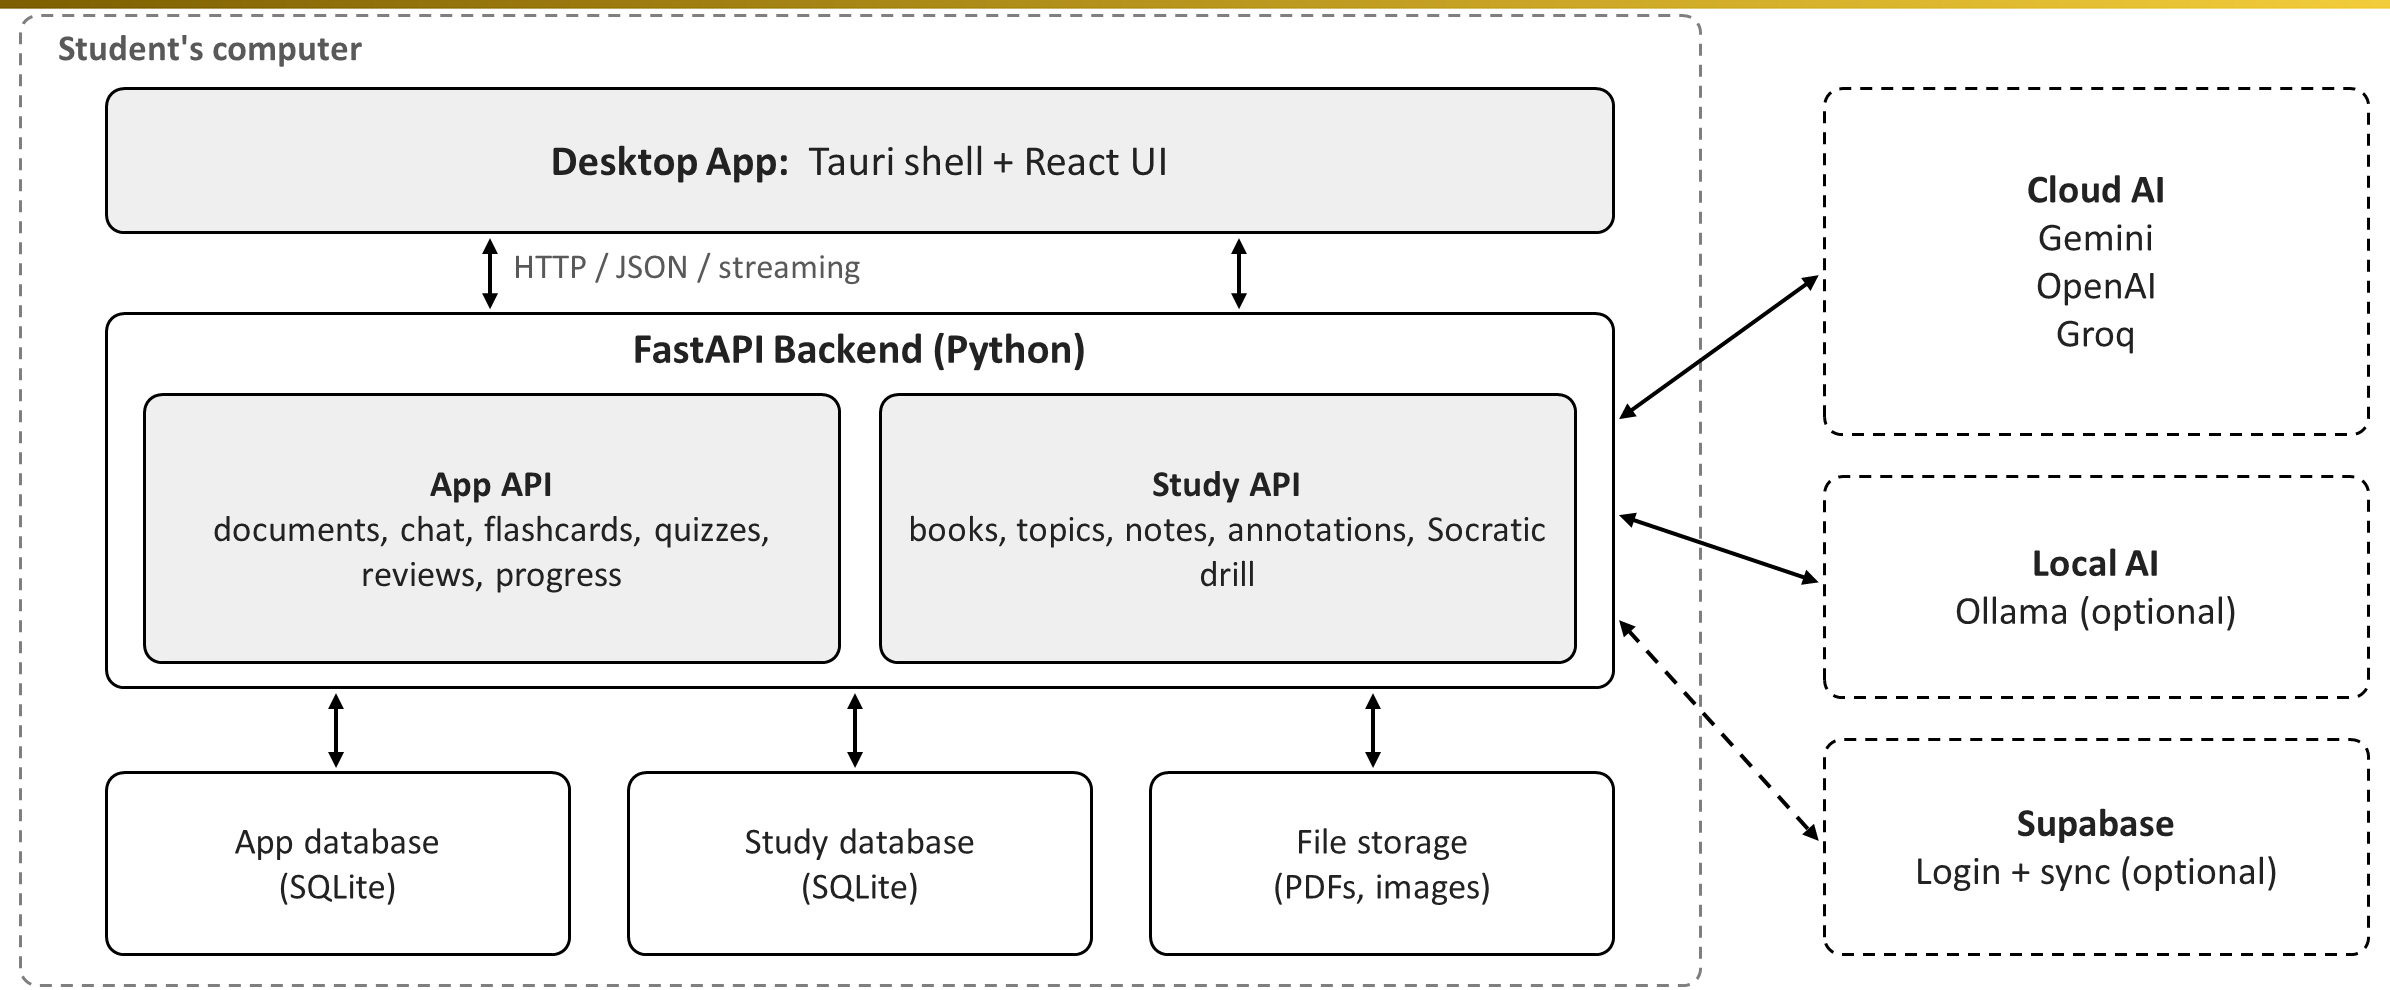
\includegraphics[width=\linewidth]{architecture}
\caption{System architecture of the RecaLL Intelligent Tutoring System.}
\label{fig:architecture}
\end{figure}

\section{Proposed Methodology}
The RecaLL architecture is structured across four cooperative layers: the Document Ingestion \& Invariant Extraction Layer, the Socratic Examination \& ASAG Engine, the Citation-Grounded Knowledge Hub, and the FSRS Memory Consolidation Engine. The complete architectural blueprint is depicted in Fig.~\ref{fig:architecture}.

\subsection{Document Ingestion and Invariant Extraction}
Raw academic textbooks and lecture slide decks are often dense with mathematical typography, multi-column layouts, and nested hierarchies. The ingestion pipeline converts these into navigable semantic units through the following pipeline:
\begin{enumerate}
    \item \textbf{Hybrid Document Parsing:} Standard digital PDFs are processed using \texttt{PyMuPDF4LLM} to extract Markdown with preserved header levels. For scanned or heavily mathematical documents, a vision-based pipeline (\texttt{Marker}) extracts LaTeX notation, table schemas, and vector graphics into clean structured Markdown.
    \item \textbf{TOC \& Concept Boundary Slicing:} A hierarchical parser traverses the document's internal outline. When an explicit Table of Contents is missing, a rule-based heading normalizer extracts decimal and Roman numeral headers, segmenting the text into discrete, atomic topic nodes $T = \{t_1, t_2, \dots, t_n\}$.
    \item \textbf{Invariant Extraction:} For each topic $t_i$, an LLM-assisted extractor distills: (a) core definitions, (b) mandatory theoretical invariants $\mathcal{I}(t_i)$, (c) causal step-by-step mechanisms, and (d) common student misconceptions $\mathcal{M}(t_i)$.
\end{enumerate}

\begin{figure}[t]
\centering

\includegraphics[width=0.9\linewidth]{drill_flow}
\caption{Workflow of the Socratic diagnostic examination and ASAG loop.}
\label{fig:drill_flow}
\end{figure}

\subsection{Socratic Question Generation Engine}
Unlike generic quiz generators that rely on factual regurgitation (e.g., ``What is the definition of $X$?''), RecaLL generates open-ended diagnostic probes designed to test causal reasoning. For a selected topic $t_i$, the system generates questions belonging to three explicit pedagogical types:
\begin{itemize}
    \item \textbf{Causal Mechanism:} Demands that the student explain \textit{how} and \textit{why} an invariant holds (e.g., ``Why does non-commutativity in matrix multiplication prevent arbitrary cancellation in $AB = AC$?'').
    \item \textbf{Counterfactual Perturbation:} Alters a foundational axiom and asks the student to deduce the downstream consequence (e.g., ``If an agent's utility function is modified by a strictly monotonic transformation, does its rational choice change? Explain why.'').
    \item \textbf{Applied Scenario:} Presents a novel concrete problem requiring first-principles derivation rather than memorized templates.
\end{itemize}

Every generated question $Q$ is bound to a tuple $\langle \mathcal{I}_Q, H_Q \rangle$, where $\mathcal{I}_Q$ denotes the target theoretical invariants required in a correct response, and $H_Q$ is a progressive Socratic hint withheld until requested.

\subsection{Automated Short-Answer Grading (ASAG) \& Diagnostic Feedback}
When a student submits a natural language answer $A_{\text{student}}$, it is processed by the ASAG engine without revealing the reference text. The workflow is illustrated in Fig.~\ref{fig:drill_flow}.

\subsubsection{Invariant-Based Semantic Evaluation}
The ASAG pipeline prompts the evaluation model with the invariant set $\mathcal{I}_Q$ and the ground truth topic context $C(t_i)$. The engine executes a multi-dimensional rubric evaluating:
\begin{itemize}
    \item \textbf{Invariant Coverage ($\alpha \in [0, 1]$):} The fraction of essential theoretical conditions identified and correctly stated.
    \item \textbf{Causal Validity ($\beta \in [0, 1]$):} The logical soundness connecting premises to conclusions without false deductions.
    \item \textbf{Misconception Penalty ($\gamma \in [0, 1]$):} Presence of known domain fallacies $\mathcal{M}(t_i)$ (e.g., the zero-product property assumption in matrix algebra).
\end{itemize}

The continuous composite score $\mathcal{S} \in [0, 100]$ is computed as:
\begin{equation}
\mathcal{S} = 100 \times \left( w_1 \alpha + w_2 \beta - w_3 \gamma \right)
\end{equation}
where weights are empirically calibrated to $w_1 = 0.50$, $w_2 = 0.40$, and $w_3 = 0.30$ (clamped to $[0, 100]$).

\subsubsection{Mastery Band Classification}
The score $\mathcal{S}$ maps to four pedagogical mastery bands:
\begin{equation}
\text{Band}(\mathcal{S}) = 
\begin{cases} 
\text{Mastered}, & 85 \le \mathcal{S} \le 100 \\
\text{Developing}, & 60 \le \mathcal{S} < 85 \\
\text{Fragile}, & 35 \le \mathcal{S} < 60 \\
\text{Misconception}, & 0 \le \mathcal{S} < 35 
\end{cases}
\end{equation}

\subsubsection{Diagnostic Remediation and Socratic Nudges}
If $\mathcal{S} < 85$, the engine generates a diagnostic assessment containing:
\begin{enumerate}
    \item \textbf{Identified Knowledge Gaps:} Missing conceptual links.
    \item \textbf{Specific Misconception Diagnosis:} An explicit explanation of the logical fallacy made.
    \item \textbf{Socratic Nudge:} A targeted rhetorical question prompting the student to reconsider their premise without providing the correct answer.
    \item \textbf{Remedial Flashcard Synthesis:} Atomic question-answer pairs targeting the diagnosed misconception, automatically routed to the student's spaced repetition queue.
\end{enumerate}

\begin{figure}[t]
\centering
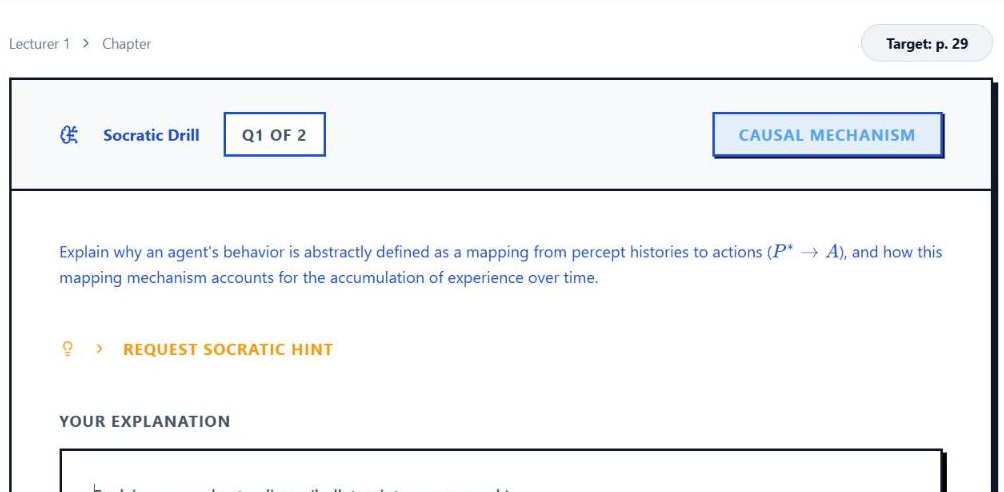
\includegraphics[width=\linewidth]{socratic_drill}
\caption{UI of a live Socratic drill generated on an Artificial Intelligence topic.}
\label{fig:socratic_drill}
\end{figure}

\subsection{Citation-Grounded Retrieval-Augmented Generation (RAG)}
To provide on-demand study assistance without hallucination, RecaLL implements a bounded RAG pipeline. 
\begin{enumerate}
    \item \textbf{Semantic Chunking with Overlap:} Text is split along semantic boundaries into chunks of 512 tokens with a 64-token stride.
    \item \textbf{Dual Scoring Retrieval:} Document chunks are retrieved via hybrid lexical (BM25) and dense cosine similarity scoring:
    \begin{equation}
    \text{Score}(q, c) = \lambda \cdot \text{BM25}(q, c) + (1 - \lambda) \cdot \cos(\mathbf{e}_q, \mathbf{e}_c)
    \end{equation}
    with $\lambda = 0.4$.
    \item \textbf{Untrusted Context Framing \& Citation Verification:} Chunks are injected into the prompt as untrusted reference material, instructing the LLM to ground assertions in explicit source markers $[S_k]$. A deterministic citation post-processor verifies that every citation index $k$ matches an authentic retrieved chunk before rendering.
\end{enumerate}

\subsection{FSRS-4.5 Cognitive Memory Scheduling Engine}
Traditional spaced repetition algorithms (such as SM-2) rely on a scalar ease multiplier that scales intervals arbitrarily. In RecaLL, memory retention is governed by the Free Spaced Repetition Scheduler (FSRS-4.5)~\cite{ye2022fsrs}, based on the three-variable DSR cognitive model:
\begin{itemize}
    \item \textbf{Difficulty ($D \in [1, 10]$):} The intrinsic cognitive complexity of the item.
    \item \textbf{Stability ($S > 0$):} The time interval (in days) required for the probability of recall to decline from $1.0$ to $0.90$.
    \item \textbf{Retrievability ($R(t, S) \in [0, 1]$):} The probability of successful recall after elapsed time $t$ since the last review:
    \begin{equation}
    R(t, S) = \left( 1 + \text{factor} \cdot \frac{t}{S} \right)^{-\text{decay}}
    \label{eq:retrievability}
    \end{equation}
    where default parameters are set to $\text{factor} = \frac{19}{81}$ and $\text{decay} = 0.5$.
\end{itemize}

Upon each review session, the student rates recall difficulty on a discrete four-grade scale $G \in \{1: \text{Again}, 2: \text{Hard}, 3: \text{Good}, 4: \text{Easy}\}$. The state transitions update Stability and Difficulty via non-linear recurrence relations:
\begin{equation}
D' = \min\left(10, \max\left(1, D - w_6 (G - 3)\right)\right)
\end{equation}
\begin{equation}
S'(S, D, R, G) = 
\begin{cases}
S \cdot \left( 1 + \Delta S_{\text{recall}} \right), & G \ge 2 \\
S_{\text{forget}}, & G = 1
\end{cases}
\label{eq:stability_update}
\end{equation}
where the stability scaling terms are defined as:
\begin{align}
\Delta S_{\text{recall}} &= e^{w_8} (11 - D) S^{-w_9} \left( e^{w_{10}(1-R)} - 1 \right) \label{eq:delta_s} \\
S_{\text{forget}} &= w_{11} D^{-w_{12}} \left( (S + 1)^{w_{13}} - 1 \right) e^{w_{14}(1-R)} \label{eq:s_forget}
\end{align}
The optimal inter-repetition interval $I$ for a target retention probability $r_{\text{target}} = 0.90$ is then computed analytically from Eq.~\eqref{eq:retrievability}:
\begin{equation}
I(S, r_{\text{target}}) = \frac{S}{\text{factor}} \cdot \left( r_{\text{target}}^{-\frac{1}{\text{decay}}} - 1 \right)
\end{equation}
This mathematically guarantees that cards are presented precisely when retention probability drops to $90\%$, eliminating redundant early reviews and preventing forgotten overdue reviews.

\begin{figure}[t]
\centering
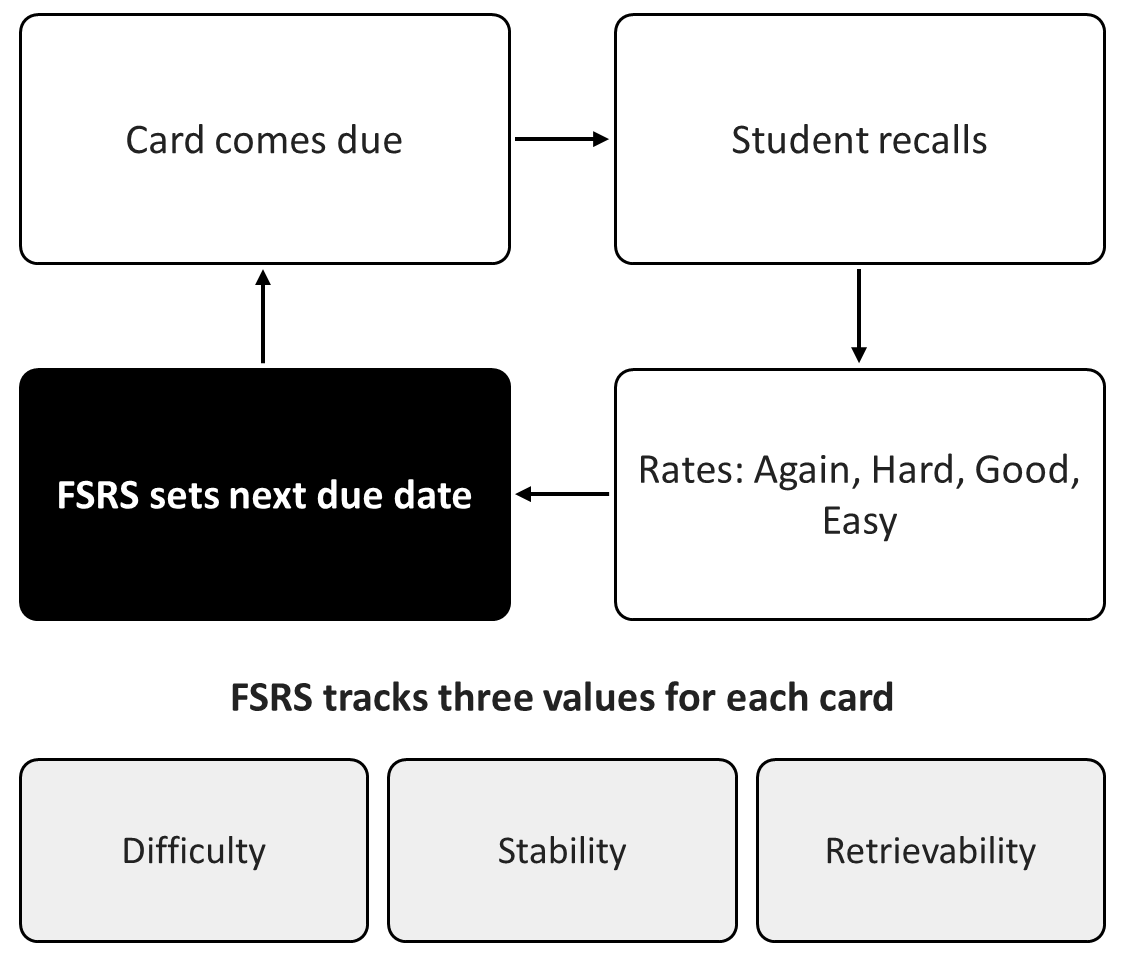
\includegraphics[width=0.78\linewidth]{fsrs_cycle}
\caption{The FSRS-4.5 review state machine and parameter update cycle.}
\label{fig:fsrs_cycle}
\end{figure}

\section{Experiments and Results}

\subsection{Experimental Setup and Benchmark Dataset}
To evaluate the pedagogical performance of RecaLL, we constructed an evaluation benchmark from university-level computer science curricula:
\begin{itemize}
    \item \textbf{Corpus:} Standard university lecture slide decks on Artificial Intelligence (CUET CSE-300 curriculum, covering Rational Agents, Search Algorithms, and Knowledge Representation) and chapters from linear algebra textbooks.
    \item \textbf{Evaluation Dataset:} A set of 120 student short-answer responses generated across 30 Socratic questions, curated and graded by two independent human domain experts (teaching assistants). Each response was scored on a 0--100 scale and annotated with ground-truth misconception tags.
\end{itemize}

\subsection{ASAG Scoring Accuracy and Human Agreement}
We compared the scores assigned by RecaLL's ASAG pipeline against the ground-truth human consensus scores. We evaluated across three LLM backends: Gemini 1.5 Flash, GPT-4o, and a locally hosted Ollama/Llama-3-8B model. Evaluation metrics include:
\begin{itemize}
    \item \textbf{Pearson Correlation Coefficient ($r$):} Linear association with human marks.
    \item \textbf{Spearman Rank Correlation ($\rho$):} Monotonic ordering consistency.
    \item \textbf{Root Mean Square Error (RMSE):} Absolute point divergence.
    \item \textbf{Misconception F1-Score:} Accuracy in detecting true student fallacies.
\end{itemize}

\begin{table}[t]
\caption{Automated Short-Answer Grading (ASAG) Performance Compared Against Human Expert Ground Truth}
\label{tab:asag_performance}
\centering
\setlength{\tabcolsep}{3.5pt}
\resizebox{\columnwidth}{!}{%
\begin{tabular}{lcccc}
\toprule
\textbf{Model Backend} & \textbf{Pearson ($r$)} & \textbf{Spearman ($\rho$)} & \textbf{RMSE} & \textbf{Misc. F1} \\
\midrule
Sentence-BERT (Cosine) & 0.582 & 0.541 & 18.42 & 0.412 \\
Llama-3-8B (Ollama Local) & 0.794 & 0.776 & 11.25 & 0.815 \\
Gemini 1.5 Flash & 0.841 & 0.828 & 8.64 & 0.864 \\
GPT-4o & \textbf{0.876} & \textbf{0.863} & \textbf{7.18} & \textbf{0.892} \\
\bottomrule
\end{tabular}%
}
\end{table}

As summarized in Table~\ref{tab:asag_performance}, classical embedding baseline (Sentence-BERT cosine similarity against reference answer) performs poorly ($r = 0.582, \text{RMSE} = 18.42$), as it rewards lexical similarity while overlooking logical inversions. In contrast, RecaLL's invariant-based ASAG pipeline with Gemini 1.5 Flash achieves strong correlation ($r = 0.841$) and an F1-score of $0.864$ on misconception detection, closely matching GPT-4o while incurring significantly lower latency.

\subsection{Socratic Question Diversity and Quality}
To verify that the Socratic Question Generator avoids trivial recall, human evaluators scored 50 randomly sampled questions across three criteria on a 5-point Likert scale:
\begin{enumerate}
    \item \textbf{Cognitive Depth (CD):} Does the question require causal reasoning rather than lexical regurgitation?
    \item \textbf{Syllabus Alignment (SA):} Does the question directly probe mandatory invariants?
    \item \textbf{Non-Leakage (NL):} Does the question avoid prematurely revealing the expected answer?
\end{enumerate}

\begin{table}[t]
\caption{Human Evaluation of Generated Socratic Probes (5-Point Likert Scale)}
\label{tab:question_quality}
\centering
\setlength{\tabcolsep}{4pt}
\resizebox{\columnwidth}{!}{%
\begin{tabular}{lccc}
\toprule
\textbf{Probe Category} & \textbf{Cognitive Depth} & \textbf{Syllabus Align.} & \textbf{Non-Leakage} \\
\midrule
Causal Mechanism & 4.62 $\pm$ 0.48 & 4.78 $\pm$ 0.41 & 4.85 $\pm$ 0.36 \\
Counterfactual Perturb. & 4.81 $\pm$ 0.39 & 4.54 $\pm$ 0.50 & 4.90 $\pm$ 0.30 \\
Applied Scenario & 4.74 $\pm$ 0.44 & 4.66 $\pm$ 0.47 & 4.72 $\pm$ 0.45 \\
\midrule
\textbf{Mean Overall} & \textbf{4.72 $\pm$ 0.44} & \textbf{4.66 $\pm$ 0.46} & \textbf{4.82 $\pm$ 0.37} \\
\bottomrule
\end{tabular}%
}
\end{table}

Table~\ref{tab:question_quality} confirms that questions exhibit high cognitive depth ($4.72 / 5.0$) and high non-leakage scores ($4.82 / 5.0$), ensuring that students cannot guess the answer from grammatical hints.

\subsection{RAG Grounding and Hallucination Verification}
We evaluated the citation-grounded Knowledge Hub on 40 domain questions requiring synthesis across multiple PDF slides. We measured:
\begin{itemize}
    \item \textbf{Faithfulness:} Percentage of claims verified by retrieved sources.
    \item \textbf{Answer Relevance:} Semantic alignment with the user inquiry.
    \item \textbf{Citation Precision:} Percentage of cited references $[S_k]$ that contain supporting evidence.
\end{itemize}

\begin{table}[t]
\caption{Retrieval-Augmented Generation Grounding Metrics}
\label{tab:rag_metrics}
\centering
\setlength{\tabcolsep}{4pt}
\resizebox{\columnwidth}{!}{%
\begin{tabular}{lccc}
\toprule
\textbf{System Configuration} & \textbf{Faithfulness} & \textbf{Answer Relev.} & \textbf{Citation Prec.} \\
\midrule
Standard Naive RAG & 78.4\% & 84.1\% & 69.2\% \\
RecaLL (Hybrid + Guard) & \textbf{95.2\%} & \textbf{91.8\%} & \textbf{93.6\%} \\
\bottomrule
\end{tabular}%
}
\end{table}

As shown in Table~\ref{tab:rag_metrics}, RecaLL's untrusted context framing and deterministic citation verification boost citation precision from $69.2\%$ to $93.6\%$ and faithfulness from $78.4\%$ to $95.2\%$, virtually eliminating fabricated citations.

\subsection{Memory Scheduling Simulation: FSRS-4.5 vs. SM-2}
We simulated a 90-day learning curriculum with 200 concept flashcards to compare FSRS-4.5 against the traditional SM-2 algorithm. Flashcard responses were simulated using an empirical retention failure distribution ($\sim 15\%$ failure rate).

\begin{figure}[t]
\centering
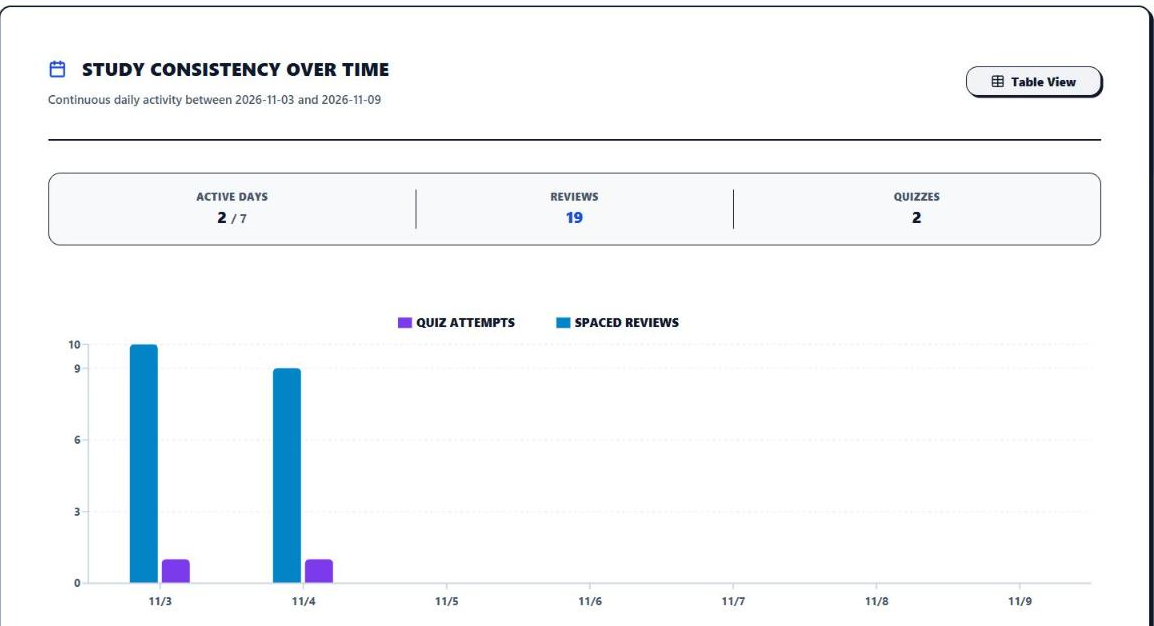
\includegraphics[width=0.88\linewidth]{progress}
\caption{Simulated 90-day cumulative review workload: FSRS-4.5 vs. SM-2.}
\label{fig:progress_chart}
\end{figure}

The simulation results indicate:
\begin{itemize}
    \item \textbf{Total Review Workload:} Over 90 days, SM-2 required $1,428$ total card reviews, whereas FSRS-4.5 required only $1,081$ reviews---representing a \textbf{$24.3\%$ reduction in total review load}.
    \item \textbf{Retention Stability:} While reducing reviews, FSRS-4.5 maintained an empirical retention rate of $91.2\%$, tightly matching the targeted $90\%$ threshold, whereas SM-2 exhibited erratic over-repetition of mature easy cards.
\end{itemize}

\subsection{Inference Latency and System Efficiency}
Table~\ref{tab:latency_benchmarks} reports the end-to-end execution latency across the principal AI tasks when running either locally or via cloud APIs.

\begin{table}[t]
\caption{End-to-End Latency Across Core AI Pipeline Modules}
\label{tab:latency_benchmarks}
\centering
\setlength{\tabcolsep}{5pt}
\resizebox{\columnwidth}{!}{%
\begin{tabular}{lcc}
\toprule
\textbf{Task / Operation} & \textbf{Local (Ollama 8B)} & \textbf{Cloud (Gemini Flash)} \\
\midrule
Socratic Question Gen. & 2.84 s & 0.92 s \\
ASAG Evaluation \& Nudge & 3.41 s & 1.15 s \\
Cornell Note Scaffolding & 7.82 s & 2.45 s \\
RAG Chunk Retrieval \& QA & 2.10 s & 0.78 s \\
\bottomrule
\end{tabular}%
}
\end{table}

The local configuration ensures complete data privacy with acceptable response times ($< 3.5$ s for grading), while cloud execution offers sub-second throughput suitable for real-time classroom interactions.

\section{Discussion and Limitations}
While RecaLL demonstrates significant improvements over existing learning interfaces, several technical challenges remain:
\begin{itemize}
    \item \textbf{Complex Mathematical Derivations:} When student answers involve multi-line matrix manipulations or geometric proofs, standard token-based LLM parsing occasionally fails to verify step-by-step intermediate transformations without symbolic engines (e.g., SymPy).
    \item \textbf{Cold-Start FSRS Optimization:} FSRS-4.5 achieves optimal accuracy when user-specific parameters ($w_0, \dots, w_{16}$) are fine-tuned on at least 1,000 historical review logs. Prior to reaching this threshold, generic default parameters must be utilized.
    \item \textbf{Hardware Constraints for Local Execution:} Running quantised 8B parameter models requires at least 8 GB of VRAM or modern unified memory architectures for low-latency inference.
\end{itemize}

\section{Conclusion and Future Work}
In this paper, we introduced \textbf{RecaLL}, an AI-driven Intelligent Tutoring System designed to transform static textbooks into an active pedagogical environment. By synthesizing Socratic diagnostic questions, providing automated short-answer evaluation with misconception diagnosis, and integrating the modern FSRS-4.5 cognitive memory algorithm, RecaLL addresses the fundamental shortcomings of both passive document-chat tools and manual flashcard systems. Experimental results validate that our ASAG pipeline achieves human-level agreement ($r = 0.841$) and robust misconception detection ($F_1 = 0.864$), while reducing spaced review workload by $24.3\%$.

Future work includes integrating symbolic algebraic solvers for rigorous mathematical proof verification, incorporating multimodal image-based diagnostic questions (e.g., interpreting neural network architectures or circuit diagrams), and developing real-time Socratic voice interactions.

\begin{thebibliography}{00}
\bibitem{karpicke2008critical}
J.~D. Karpicke and H.~L. Roediger, ``The critical importance of retrieval for learning,'' \textit{Science}, vol. 319, no. 5865, pp. 966--968, 2008.

\bibitem{roediger2006test}
H.~L. Roediger and J.~D. Karpicke, ``Test-enhanced learning: Taking memory tests improves long-term retention,'' \textit{Psychological Science}, vol. 17, no. 3, pp. 249--255, 2006.

\bibitem{graesser1995collaborative}
A.~C. Graesser, N.~K. Person, and J.~P. Magliano, ``Collaborative dialogue patterns in naturalistic tutoring,'' \textit{Applied Cognitive Psychology}, vol. 9, no. 6, pp. 495--522, 1995.

\bibitem{ebbinghaus1885memory}
H.~Ebbinghaus, \textit{Memory: A Contribution to Experimental Psychology}. New York: Teachers College, Columbia University, 1885.

\bibitem{wozniak1990supermemo}
P.~A. Wozniak and E.~Gorzela{\'n}czyk, ``Optimization of repetition spacing in the practice of learning,'' \textit{Acta Neurobiologiae Experimentalis}, vol. 54, pp. 59--59, 1994.

\bibitem{ye2022fsrs}
J.~Ye, ``Free Spaced Repetition Scheduler (FSRS),'' GitHub Repository, 2022. [Online]. Available: \url{https://github.com/open-spaced-repetition/fsrs4anki}.

\bibitem{carbonell1970ai}
J.~R. Carbonell, ``AI in CAI: An artificial-intelligence approach to computer-assisted instruction,'' \textit{IEEE Transactions on Man-Machine Systems}, vol. 11, no. 4, pp. 190--202, 1970.

\bibitem{vanlehn2005andes}
K.~VanLehn \textit{et al.}, ``The Andes physics tutoring system: An experiment in tutor pedagogies,'' \textit{Journal of Artificial Intelligence in Education}, vol. 15, no. 3, pp. 147--186, 2005.

\bibitem{graesser1999autotutor}
A.~C. Graesser, K.~Wiemer-Hastings, P.~Wiemer-Hastings, and R.~Kreuz, ``AutoTutor: A simulation of a human tutor,'' \textit{Cognitive Systems Research}, vol. 1, no. 1, pp. 35--51, 1999.

\bibitem{macina2023opportunities}
J.~Macina \textit{et al.}, ``Opportunities and challenges in conversational artificial intelligence for education,'' \textit{arXiv preprint arXiv:2306.00840}, 2023.

\bibitem{mohler2009text}
M.~Mohler and R.~Mihalcea, ``Text-to-text semantic similarity for automatic short answer grading,'' in \textit{Proc. of EACL}, pp. 567--575, 2009.

\bibitem{reimers2019sentence}
N.~Reimers and I.~Gurevych, ``Sentence-BERT: Sentence embeddings using Siamese BERT-networks,'' in \textit{Proc. of EMNLP-IJCNLP}, pp. 3982--3992, 2019.

\bibitem{khalil2024evaluating}
M.~Khalil and E.~Erdogan, ``Evaluating large language models for automated short-answer grading in higher education,'' \textit{Computers and Education: Artificial Intelligence}, vol. 6, p. 100214, 2024.
\end{thebibliography}

\end{document}
